\chapter{Technische aspecten}
\section{Machine Learning}
\subsection{Inleiding}
\npar Leren is een veelzijdig fenomeen dat bestaat uit  verschillende processen: het verkrijgen van declaratieve kennis, het ontwikkelen van motorische en cognitieve vaardigheden door instructie en ervaring, het organiseren van nieuwe kennis in algemene representaties en het ontdekken van nieuwe feiten via observatie en experimentatie.
\npar Sinds het begin van het computertijdperk proberen onderzoekers het menselijk leren na te bootsen en deze processen te vertalen naar de informatietheorie. Het machinaal leren is nog steeds een erg uitdagend doel in de kunstmatige intelligentie (KI).

\npar Deze vorm van KI is dus volledig data gedreven tegenover traditionele methoden die zich beroepen op handgemaakte regels. Het computerprogramma wordt niet expliciet geprogrammeerd om een taak uit te voeren maar vertrekt vanuit een algemeen model. Het model leert eerst uit voorbeelden en kan daarna voorspellingen maken op nieuwe invoer.

\npar We kunnen zeggen dat een computerprogramma of machine leert als het zijn performantie op een bepaalde taak verbetert met ervaring \cite{machine_overview}.  Het leren gebeurt door de optimalisatie van de parameters van het predictief model door middel van een algoritme uit de machine learning. Het model wordt een aantal voorbeelden gegeven om uit te leren: de trainset. De uitvoer van het model wordt ge\"evalueerd aan de hand van een prestatiemaat. Deze prestatiemaat vertelt hoe correct de voorspelling is en bepaalt de mate waarin het model verder gecorrigeerd dient te worden.

\npar Machine learning algoritmes kunnen opgedeeld worden in drie categori\"en op basis van leerstijl: gesuperviseerd, ongesuperviseerd en semi-gesuperviseerd leren. De supervisie slaat op het gebruik van de correcte uitgangswaarde tijdens het trainen.

\npar Een ongesuperviseerde leerstijl vertrekt uit een dataset zonder klasselabels of correcte voorspellingswaarde. Er wordt een model opgebouwd die bepaalde structuren deduceert. Dit kan zijn om algemene regels te extraheren, om redundantie te verminderen of om gegevens te groeperen volgens gelijkenis (clustering).

\npar Bij gesuperviseerde methodes wordt een trainset gebruikt die zowel de invoervector als de te voorspellen waarde bevat. Problemen die vaak via gesuperviseerd leren worden aangepakt zijn classificatie en regressie. Classificatie tracht ingevoerde voorbeelden in te delen in discrete categori\"en om bijvoorbeeld objecten te herkennen zoals in \cite{krizhevsky2012imagenet}. Bij regressie is de uitvoer van het model een continue variabele zoals bijvoorbeeld de prijs van een appartement gegeven zijn oppervlakte.

\npar Semi-gesuperviseerde methodes zijn een mengvorm van de voorgaande twee. De dataset is een mengeling van gelabelde en ongelabelde voorbeelden. Hierbij is er een gewenste indeling, weergegeven door de gelabelde data, maar het model moet zelf de indeling zien te maken.


\subsection{Gesuperviseerde classificatie}

\npar De machine learning in dit onderzoek valt onder de gesuperviseerde classificatie. Een classificatieprobleem kan algemeen als volgt worden omschreven:
\npar Gegeven een trainset T:
\begin{equation}
T = \{ ( x^{(n)}, y^{(n)})\},\quad x^{(n)}\in\mathbb{R}^D, y^{(n)}\in\{0,1,...,C\}, n=1,...,N
\end{equation}
met $x^{(n)}$ het n-de datavoorbeeld en $y^{(n)}$ zijn klasselabel. C staat voor het aantal discrete categori\"en of klasses, D het aantal dimensies van de invoervariabelen en N het aantal trainingsvoorbeelden. Nu kunnen we het classificatieprobleem uitdrukken als de benadering van een model $f$ met parameters $\theta$:
\begin{equation}\label{eq:classifier}
f(x,\theta) = y,\quad\forall(x,y) \in T
\end{equation}
zodat we na deze schatting vanuit $f$ en $\theta$ voorspellingen kunnen maken op basis van nieuwe data: $f(x_{nieuw},\theta)=y', \quad y' \in\{0,1,...C\}$

\npar Figuur \ref{fig:alg-class-model} geeft een schematische weergave van de opbouw van een classificatiemodel. Het schatten van $f$ en $\theta$ wordt uitgevoerd door een techniek uit de machine learning en geeft ons het uiteindelijke predictief model $f(x,\theta) = y$. De samples worden meestal verwerkt voor ze als input worden doorgegeven aan het model. In het geval van classificatie van video en afbeeldingen worden er technieken uit de beeldverwerking gebruikt om relevante informatie uit het beeld te halen. Welke specifieke techniek er gebruikt wordt is een keuze die erg bewust moet gemaakt worden en een grote invloed heeft op de performantie van het classificatiemodel. Deze informatie wordt gebundeld in een featurevector ($x$) en aan het ML algoritme gegeven. Vanuit de verkregen featurevectoren en de kennis van het correcte klasselabel wordt het predictief model dan geoptimaliseerd.
\npar Eenmaal het model voldoende geleerd heeft kan het predictief model gebruikt worden in een productieomgeving om nieuwe voorbeelden, al dan niet correct, te classificeren.
\npar Het model dat in dit onderzoek gebruikt wordt is dat van het artificieel neuraal netwerk, een veel gebruikt predictief model voor classificatie. In sectie \ref{sec:ann} wordt deze techniek dan ook verder besproken.
\begin{figure}[t]
	\centering
	\def\svgscale{0.85}
%	\def\svgwidth{\columnwidth}
	\input{figuren/figuur-classificatieML.pdf_tex}
	\caption{Schematische weergave van het opstellen van een predictief model met behulp van machine learning technieken \label{fig:alg-class-model}}
\end{figure}

\subsection{Overfitting}
Stel dat een student kunstwetenschappen voor zijn examen het werk van verschillende kunstenaars moet herkennen. Hij krijgt een boek met daarin foto's van verschillende schilderijen samen met de naam van de uitvoerder. Indien de student al deze voorbeelden met hun antwoord vanbuiten leert en op het examen net dezelfde schilderijen als in het boek zou voorgeschoteld krijgen, dan zal hij erg hoog scoren. Krijgt hij echter ongeziene werken van dezelfde schilders, dan zal zijn score veel lager liggen. Hij heeft geen onderliggende eigenschappen uit de beelden gehaald die terugkomen in ander werk maar memoriseerde gewoon werk en uitvoerder dus heeft hij veel moeite met het categoriseren van de nieuwe voorbeelden. Dit is een informeel voorbeeld van overfitting.

\npar Bij overfitting beschrijft het predictief model de ruis en fouten in het signaal in plaats van de gewenste onderliggende patronen en kenmerken van de gegeven taak. Het komt voor wanneer het model complex is en vele parameters heeft in vergelijking met het aantal trainingsvoorbeelden. Een model dat ``overfit'' is heeft een laag voorspellend vermogen op ongeziene data. Het model is niet algemeen of gegeneraliseerd en  memoriseert de data. 

\begin{figure}
	\centering
	\def\svgscale{0.7}
	%	\def\svgwidth{\columnwidth}
	\input{figuren/overfitting.pdf_tex}
	\caption{Plot van trainings- en validatiefout ter illustratie van overfitting en de early stopping techniek.}
	\label{fig:overfitting}
\end{figure}

\npar Het risico op overfitten komt uit het feit dat de prestatiemaat voor de training van het model niet correct de effectiviteit van het model weergeeft. De training van een model gebeurt doorgaans via optimalisatie van zijn prestatie op een training set. De werkelijke performantie wordt echter gegeven door prestatie op ongeziene data. Net om deze reden wordt de dataset opgesplitst in drie delen: training-, validatie- en testset.
\npar Om een zo goed mogelijk predictief model te maken wordt een evaluatiescore op de validatieset geminimaliseerd of gemaximaliseerd. Deze data is nog onbekend voor het model en geeft dus een betere aanduiding van zijn performantie. Figuur \ref{fig:overfitting} geeft de validatie- en trainingsfout weer tijdens het trainen van een predictief model. Wanneer de trainingsfout blijft dalen maar de validatiefout stagneert of stijgt is er sprake van overfitting. Nu kan er gekozen worden om de training vroegtijdig te stoppen teneinde geen generalisatie te verliezen. Deze techniek wordt \textit{early stopping} genoemd.

\npar Om na afloop een finale evaluatie van het model te maken wordt zijn prestatie op de testset gemeten. Het model heeft de voorbeelden uit deze set nog nooit eerder gezien waardoor de testscore representatief is voor het voorspellingsvermogen van het model. De testset mag nooit gebruikt worden om aanpassingen aan het model te maken, hiervoor dient de validatieset.

\section{Artificieel neuraal netwerk}\label{sec:ann}
\subsection{Inleiding}
\begin{figure}
	\centering
	\begin{subfigure}{.5\textwidth}
		\centering
		\input{figuren/neuron.pdf_tex}
		\caption{Artificieel neuron.}
		\label{fig:neuron}
	\end{subfigure}%
	\begin{subfigure}{.5\textwidth}
		\centering
		\input{figuren/ANN-alg.pdf_tex}
		\caption{Artificieel neuraal netwerk}
		\label{fig:ANN}
	\end{subfigure}
	\caption{Een ANN met een invoerlaag, twee verborgen lagen en een softmax uitvoerlaag samen met zijn bouwsteen, het artificieel neuron.}
	\label{fig:test}
\end{figure}
Een lange rekensom uitwerken is iets wat de mens liever overlaat aan een rekenmachine of computer. Alle bits van een rekensom zijn even belangrijk en bepalend voor zijn uitkomst. Op dit vlak is een computer veel effici\"enter en betrouwbaarder dan ons brein. Onze hersenen zijn veel bedrevener in andere taken zoals het indelen van objecten volgens gelijkenis of het herkennen van een persoon.
\npar Het is deze gedachte die vele onderzoekers ertoe bracht een artificieel neuraal netwerk (ANN) uit te bouwen. Het menselijke brein is een erg complex neuraal netwerk bestaande uit meer dan 86 miljard neuronen. Dit zijn de bouwstenen van ons zenuwstelsel en ze staan in voor het verwerken en overdragen van informatie. In figuur \ref{fig:neuron} is een weergave te zien van een artificieel neuron, de bouwsteen van het ANN. De functionaliteit van dit neuron bootst deze van het biologisch neuron na en wordt als volgt gedefini\"eerd:
\begin{equation}\label{eq:neuron}
n = a\bigg(b+\sum_{i=1}^{D}w_ix_i\bigg)
\end{equation}
met $n$ de uitvoer van het neuron, $a$ de \textit{activatiefunctie}, $b$ de bias, $x_i$ de $i$-de invoer en $w_i$ de gewichten van zijn respectievelijke inkomende verbindingen.



\npar Deze artifici\"ele neuronen worden gegroepeerd in lagen om een ANN te vormen zoals afgebeeld in figuur \ref{fig:ANN}. Alle lagen worden onderling volledig verbonden, elk neuron krijgt invoer van alle neuronen uit de voorgaande laag en geeft zijn uitvoer door aan alle neuronen van de volgende laag. Deze lagen worden dan ook vaak \textit{dense layers} genoemd vanwege hun verbindingsdichtheid.
\npar Hier beschouwen we enkel \textit{feedforward neurale netwerken}. Aan het begin van het netwerk hebben we de invoerlaag met evenveel knopen als de dimensie van de featurevectoren. De invoer propageert zich van links naar rechts door het netwerk tot het bij de uitvoerlaag komt. Omdat de uitvoer van de binnenste lagen niet meteen zichtbaar is worden deze de verborgen lagen genoemd.
\npar De uitvoer van de verschillende lagen uit het ANN in figuur \ref{fig:ANN} kunnen we als volgt beschrijven:
\begin{equation}
\begin{aligned}
h^{(1)}_j\quad=&\quad a\bigg(b^{(1)}+\sum_{i=1}^{D}w^{(1)}_{i,j}x_i\bigg),\quad j=1,...,M_1\\
h^{(2)}_j\quad=&\quad a\bigg(b^{(2)}+\sum_{i=1}^{M_1}w^{(2)}_{i,j}h^{(1)}_i\bigg),\quad j=1,...,M_2\\ 
y_j\quad=&\quad a\bigg(b^{(3)}+\sum_{i=1}^{M_2}w^{(3)}_{i,j}h^{(2)}_i\bigg),\quad j=1,...,C 
\end{aligned}
\end{equation}
met $D$ het aantal invoerparameters, $M_1$ het aantal verborgen knopen in de eerste laag, $M_2$ het aantal verborgen knopen in de tweede laag en $C$ het aantal te voorspellen klassen. $M_1$ en $M_2$ zijn hyperparameters van het model die geoptimaliseerd worden door de evaluatie van het model tegenover de validatieset.
\npar Het is mogelijk en wenselijk om nog meer verborgen lagen toe te voegen. Het omkaderde gedeelte in figuur \ref{fig:ANN} kan een aantal keer herhaald worden om zo het model toe te laten een complexere structuur te modelleren.
\begin{figure}[ht]
	\begin{center}
		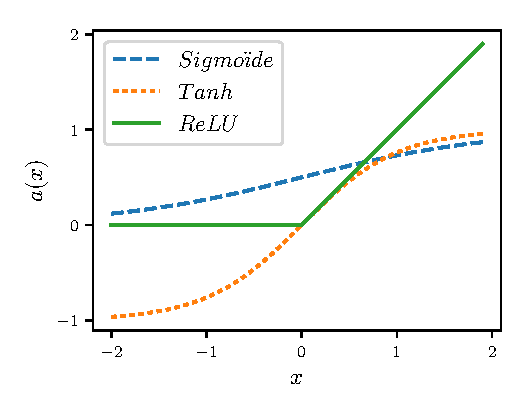
\includegraphics[width=8cm,keepaspectratio]{figuren/activatiefuncties.pdf}
		\caption{Weergave van de drie meest populaire activatiefuncties voor classificatie doeleinden \label{fig:activatie-fun}}
	\end{center}
\end{figure}
\npar De activatiefunctie $a(x)$ uit (\ref{eq:neuron}) is van groot belang in een ANN aangezien ze zorgt voor een niet-lineariteit. Moest deze er niet zijn kan elk neuraal netwerk met een verborgen laag vervangen worden door een model zonder aangezien de samenstelling van lineaire transformaties zelf een lineaire transformatie is. Figuur \ref{fig:activatie-fun} geeft drie van de meeste gebruikte niet lineaire activatiefuncties weer. In dit onderzoek zal gebruik gemaakt worden van de rectifier activatiefunctie:
\begin{equation}
\quad a(x) = max(0,x)
\end{equation}
Een neuron wordt vaak vernoemd naar de activatiefunctie die ze gebruikt. In dit geval spreken we van een Rectified Linear Unit (ReLU). Het gebruik van ReLU's wordt gestaafd door vele onderzoekswerken omtrent gesuperviseerde \textit{deep learning} zoals \cite{ReLU}, \cite{lionel} en \cite{wu_deep_2016}. Een ReLU zal alle negatieve waarden afbeelden op 0 en alle positieve op zichzelf.

\npar Aan de uitgang van het ANN worden geen ReLU's geplaatst maar hebben we de softmaxlaag. De uitvoer van de softmaxlaag geeft de voorspelde probabiliteit per klasse weer. Deze softmax wordt als volgt berekend:

\begin{equation}
\begin{aligned}
p(y = j | x) &= \frac{exp(\alpha(x)_j)}{\sum_{i=1}^{C}exp(\alpha(x)_i)}\\
softmax(x) &= \{p(y = 1 | x), p(y = 2 | x), ... , p(y = C | x)\}
\end{aligned}
\end{equation}

\npar $\alpha$ is de pre-activatie (waarde voor activatie) van de laatste verborgen laag, C het aantal klassen en $p(y=j|x)$ de probabiliteit dat een gegeven invoer $x$ tot de klasse met label $j$ behoort.

\npar De uitvoer van de softmaxlaag is een vector wiens som gelijk is aan 1. Om een voorspelling uit deze softmaxlaag te kiezen wordt het maximum genomen uit deze uitvoervector, de klasse met de hoogste probabiliteit. 

\subsection{Training van een neuraal netwerk}
Alle parameters $\theta$ van het netwerk (gewichten $w$ en biases $b$) worden pseudo-willekeurig gekozen. Tijdens het trainen worden deze dan iteratief aangepast om de prestatie van het predictief model te verbeteren. Dit gebeurt aan de hand van een \textit{back-propagation} algoritme. De data of het signaal van de invoer gaat eerst voorwaarts door het netwerk waarna we een voorspelling krijgen. Vervolgens wordt deze voorspelling ge\"evalueerd en zal de fout op de voorspelling vanuit het einde van het netwerk terug naar het begin propageren. Op basis van deze fout worden de gewichten aangepast en zo leert het model uit ervaring.

\npar Om de prestatie van het model te maximaliseren wordt een kostfunctie geminimaliseerd. Deze geeft een indicatie van de gemaakte voorspellingsfout door aan slechte voorspellingen een hogere kost toe te kennen. Welke kostenfunctie gebruikt wordt hangt af van de uit te voeren taak. Voor multinomiale classificatie met behulp van een softmax is \textit{categorical cross-entropy} het meest geschikt:
\begin{equation}
L(\theta) = - \frac{1}{N}\sum_{i=1}^{N}\sum_{j=1}^{C}y_{i,j}\log(p_{i,j})
\end{equation}
met $N$ het aantal voorbeelden en $C$ het aantal klassen. De probabiliteit uit de softmax wordt hier afgekort tot p. Het ware label y is weergegeven in een one-hot codering: een vector met de grootte van het aantal klassen waarvoor alle waarden $0$ zijn behalve op de index van het correcte klasselabel, daar is ze gelijk aan $1$. Bijgevolg verdwijnt de logterm bij een foute voorspelling en wordt in de kostenfunctie enkel rekening gehouden met de fout op het ware label. Door het gebruik van een negatieve log krijgen waarden dicht bij $0$ een erg hoge fout en is de fout bij $p_{i,j}=1$ gelijk aan $0$. 
\begin{figure}[!t]
	\centering
	%	\def\svgscale{0.85}
	\def\svgwidth{0.6\columnwidth}
	\input{figuren/gradiend-descent.pdf_tex}
	\caption{Visualisatie van gradient descent algoritme in een tweedimensionale parameterruimte. De zwarte lijn geeft de verschillende iteratieve stappen van het algoritme weer. Door het volgen van de steilste helling wordt een lokaal minimum van de kostfunctie gevonden.}
	\label{fig:gradient-descent}
\end{figure}
\subsection{Gradient descent}
\npar Nu moeten de parameters $\theta$ gevonden worden die de kostenfunctie minimaliseren. Het minimum van deze kostenfunctie komt immers overeen met het optimale predictief model. Om dit minimum te vinden wordt gradient descent toegepast. In Figuur \ref{fig:gradient-descent} wordt deze techniek weergegeven in een tweedimensionale parameterruimte. Het algoritme zal de parameters iteratief bijstellen door het volgen van de stijlste helling, gegeven door de gradi\"ent van de kostfunctie:
\begin{equation}\label{eq:grad-desc}
\theta = \theta - \alpha \nabla_\theta L(\theta)
\end{equation}
met $\alpha$ de leersnelheid of \textit{learning rate}. Deze learning rate is een hyperparameter van het model en bepaalt hoeveel de parameters bijgesteld worden per iteratie. Een te kleine leersnelheid zal zorgen voor een trage convergentie en bijgevolg lange trainingsfase. Een te grote leersnelheid loopt het risico voorbij lokale minima te lopen en niet te convergeren.

\npar Het gradient descent algoritme zoals weergegeven in (\ref{eq:grad-desc}) moet de foutfunctie voor alle voorbeelden berekenen om de parameters correct aan te passen. Het trainen van neurale netwerken vraagt om grote datasets en daarom kan deze fout- en gradientsberekening erg traag uitvallen. Om dit probleem aan te pakken wordt de \textit{mini-batch gradient descent} variant ge\"implementeerd:
\begin{equation}\label{eq:mini-grad-desc}
\theta = \theta - \alpha \nabla_\theta L(\theta;x_{i:i+B};y_{i:i+B})
\end{equation}
met $L(\theta;x_{i:i+B};y_{i:i+B})$ de kostfunctie van een klein gedeelte of \textit{mini-batch} van de voorbeelden en $B$ de batch-grootte. Zo bekomt men een schatting van de globale kostfunctie en kunnen er sneller stappen worden gezet. De keuze van de batch-grootte $B$ is net als de learning rate $\alpha$ een hyperparameter van het netwerk. 
\subsection{Momentum-optimalisatie voor gradient descent}
\begin{figure}[!t]
	\centering
	%	\def\svgscale{0.85}
	\def\svgwidth{0.6\columnwidth}
	\input{figuren/momentum.pdf_tex}
	\caption{Klassiek momentum (links) tegenover Nesterov's accelerated gradient (rechts) \cite{sutskever2013importance}}
	\label{fig:momentum}
\end{figure}
Als we de parameterruimte die het gradient descent algoritme afzoekt zouden vergelijken met een helling komt het in de problemen als er veel kleine putten zijn tijdens de afdaling. Het algoritme zal oscilleren tussen deze lichte hellingen, optimalisatiepad zal zigzaggen en de convergentiesnelheid van het algoritme zal sterk dalen. Ook is het meer waarschijnlijk dat het algoritme zal blijven steken in een van deze putten en niet verder afdaalt naar het minimum.
\npar \cite{botev_nesterovs_2016} beschrijft het gebruik van momentum als optimalisatie voor het gradient descent algoritme. De parameters worden ge\"update in dezelfde richting als de vorige update. Dit kan als volgt beschreven worden:
\begin{equation}
\begin{aligned}
v_{t+1} &= \mu v_{t} - \alpha\nabla_{\theta_t} L(\theta_{t})\\
\theta_{t+1} &= \theta_t + v_{t+1}
\end{aligned}
\end{equation}
met t de iteratiestap en $\mu \in[0,1]$ de momentumco\"effici\"ent. Bewegingen in dezelfde richting zullen snelheid accumuleren waardoor het optimalisatiepad over de kleine putten rolt. Er is echter nog een verbetering aan te brengen aan deze optimalisatie genaamd Nesterov's accelerated gradient (NAG):
\begin{equation}
\begin{aligned}
v_{t+1} &= \mu v_t - \alpha\nabla_{\theta_t} L(\theta_{t}+\mu_tv_t)\\
\theta_{t+1} &= \theta_t + v_{t+1}
\end{aligned}
\end{equation}
\npar NAG kijkt eigenlijk een stap vooruit door een afschatting van de volgende beweging te maken voor de gradientsberekening. Hiervoor wordt de huidige momentumwaarde gebruikt: $\theta_{t}+\mu_tv_t$.  In praktijk zien we dat NAG doorgaans dichter tot het lokale minimum komt dan klassiek momentum. Het verschil is doorgaans heel klein maar door het iteratieve proces cumuleren deze kleine verschillen tot een grote tijdswinst bij het gebruik van NAG.

\begin{figure}[!t]
	\centering
	\begin{subfigure}{.5\textwidth}
		\centering
		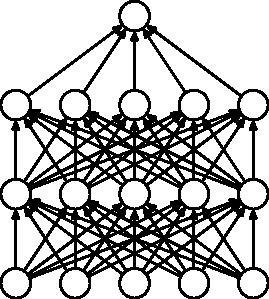
\includegraphics[width=3.5cm]{dropout-off.pdf}
		\caption{ANN}
		\label{fig:neuron}
	\end{subfigure}%
	\begin{subfigure}{.5\textwidth}
		\centering
		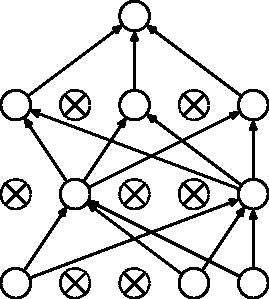
\includegraphics[width=3.5cm]{dropout-on.pdf}
		\caption{ANN na toepassing dropout}
		\label{fig:ANN}
	\end{subfigure}
	\caption{Links is een standaard ANN te zien met twee verborgen lagen, rechts is hetzelfde netwerk te zien na toepassing van dropout. De gekruiste units zijn de gedropte units.}
	\label{fig:test}
\end{figure}
\subsection{Dropout}
Tijdens het trainen kan het gebeuren dat neuronen volledig afhankelijk worden van de output van een enkel neuron uit de vorige laag (of een kleine groep neuronen). Deze units worden eigenlijk lui en dragen weinig tot niets bij aan het herkenningsvermogen. Dit fenomeen heet co-adaptatie. Om de units te verplichten zelf bij te dragen tot de herkenning van bepaalde patronen wordt dropout toegepast.
\npar Tijdens elke iteratiestap van het trainingsalgoritme worden een aantal units uitgeschakeld (vandaar de benaming dropout). Of een unit al dan niet wegvalt wordt bepaald door een probabiliteit \textit{Bernoulli(p)}. Deze $p$ is een hyperparameter van het netwerk en wordt doorgaans ingesteld op 0.5 waardoor getraind wordt met de helft van de units. Elke iteratiestap wordt er dus getraind met een andere deelverzameling neuronen, in essentie een andere netwerk. Het uitschakelen van units gebeurt enkel tijdens training, daarom worden de gewichten herschaald tijdens het trainen met een factor $1/(1-p)$. De niet geschaalde gewichten zijn bruikbaar in de testfase wanneer alle neuronen worden benut.
\npar Dropout is een regularisatiemethode die ondanks zijn simpliciteit erg effici\"ent blijkt. \cite{dropout} geeft een uitvoerige analyse en vergelijkende studie van het gebruik van dropout bij het uitvoeren van taken zoals gensplitsing, spraak-, tekst- en beeldherkenning. In elke van deze experimenen zorgt dropout voor een hogere regularisatie. Zo wordt aangetoond dat dropout overfitting kan tegengaan in om het even welk toepassingsgebied.

\section{Convolutioneel neuraal netwerk}
De machine learning techniek die sinds 2012 in de belangstelling staat is die van het convolutioneel neuraal netwerk. Mede dankzij het recordbrekende resultaat van \cite{cnn-krizhevsky} op de ``ImageNet Large Scale Visual Recognition Challenge'' wordt deze techniek vaak onderzocht en toegepast op beeldherkenningsproblemen zoals in \cite{cnn-ji} en \cite{cnn-karpathy}.
\npar Traditionele beeldherkenningstechnieken zoals in \cite{perronnin2010improving} en \cite{jhuang2007biologically} leiden het beeld af naar een manueel ontworpen beeldrepresentatie. Deze kenmerken zijn niet meteen zichtbaar maar worden via verschillende bewerkingen blootgelegd. Het is erg moeilijk om te beslissen welk soort kenmerk het best geschikt is voor de gegeven taak. Vaak moet er dan ook veelvuldig ge\"experimenteerd worden met verschillende representaties.
\begin{figure}[!t]
	\centering
	%	\def\svgscale{0.85}
	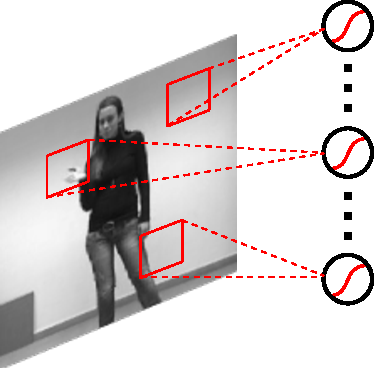
\includegraphics[width=4cm,keepaspectratio]{lokale-connectiviteit.pdf}
	\caption{Lokale connectiviteit van receptieve velden. Voor elk overlappend deelgebied van de invoer is er een neuron verbonden. Alle gewichten van het lokale filter worden gedeeld.}
	\label{fig:lokale-connectiviteit}
\end{figure}
\npar Convolutionele neurale netwerken hebben als grote troef dat ze deze feature-extractie automatiseren. CNN's zijn biologisch ge\"inspireerde model. Het onderzoek van \cite{hubel1968receptive} gaf een verklaring voor de manier waarop zoogdieren, specifiek de kat en de aap, de wereld rondom zich visueel waarnemen. De neuronen in de visuele cortex hebben een complexe laagsgewijze architectuur. Elke cel reageert op prikkels in een deelgebied van het gezichtsveld. Deze receptieve velden overlappen gedeeltelijk en bedekken zo het volledige zicht.

\npar Het herkenningsvermogen van de mens is nog altijd ontegensprekelijk veel hoger dan om het even welk artificieel herkenningssysteem. Vandaar dat er geprobeerd wordt de functionaliteit van de visuele cortex na te bootsen met een CNN. 
\npar CNN's zijn een speciaal soort meerlagig neuraal netwerk. Net zoals een ANN worden ze getraind met behulp van een back-propagation algoritme zoals beschreven in Sectie \ref{sec:leren}. Waar ze verschillen is hun architectuur. Een ANN is volledig verboden met zijn invoer. Als we een afbeelding van 64x64 pixels rechtstreeks als invoer in een ANN willen gebruiken moeten er per knoop 4096 gewichten worden getraind. De artifici\"ele neuronen in een CNN werken net zoals de receptieve velden in de visuele cortex.

\npar Zoals te zien in Figuur \ref{fig:lokale-connectiviteit} wordt elk mogelijk (overlappend) deelgebied verbonden met een neuron. De parameters van deze verbindingen worden gedeeld tussen alle units. Zo leert het netwerk een bepaalde feature detecteren om het even waar in het beeld en zijn er slechts een beperkt aantal te trainen gewichten.
 \begin{figure}[!t]
 	\centering
 	%	\def\svgscale{0.85}
 	\def\svgwidth{0.55\columnwidth}
 	\input{figuren/convolutie.pdf_tex}
 	\caption{Tweedimensionale convolutie met een 3x3 filter.}
 	\label{fig:conv}
 \end{figure}
\npar In een CNN worden convolutielagen afgewisseld met pooling lagen. Zo worden er meerdere lagen na elkaar geplaatst om een diepe architectuur te verkrijgen. In de eerste lagen zullen kenmerken van laag niveau gedetecteerd worden en naarmate we dieper in het netwerk gaan worden kenmerken van hoger niveau ge\"extraheerd. Zo zullen de eerste lagen features zoals randen detecteren die dan dieper in het netwerk worden samengesteld tot bijvoorbeeld een bepaalde handvorm.

\subsection{Tweedimensionale convolutie}

De receptieve velden delen hun parameters en zoeken dus naar hetzelfde kenmerk in een beeld. Ze filteren het beeld met behulp van een tweedimensionale discrete convolutie die als volgt kan worden beschreven:

\begin{equation}\label{eq:conv}
(w * x)_{h,b} = \sum_{b'=-\infty}^{+\infty}\sum_{h'=-\infty}^{+\infty} f_{b',h'}x_{b-b',h-h'}
\end{equation}

\npar met w de filterwaarden en x de invoer. De grootte van het filter en van de invoer is uiteraard begrensd. Met onze filtergrootte $(H_f,B_f)$ en de dimensie van onze invoer $(H_x,B_x)$ kunnen we (\ref{eq:conv}) vereenvoudigen tot:

\begin{equation}
\sum_{b'=0}^{B_f}\sum_{h'=0}^{H_f} f_{b',h'}x_{b-b',h-h'}
\end{equation}

\npar Figuur \ref{fig:conv} geeft een visuele weergave van deze convolutie operatie terug. Op het resultaat van deze operatie wordt een niet-lineaire activatiefunctie toegepast en zo bekomen we een feature-map. Let er op dat we op de randen een probleem hebben: we krijgen te grote of te kleine indices voor de input. Om dit probleem te omzeilen zijn er twee opties: de invoer uitbreiden of enkel de convolutie berekenen wanneer alle invoerwaardes gedefinieerd zijn. Deze tweede vorm heet de \textit{echte convolutie} en wordt hier toegepast. Hierdoor is de dimensie van de uitvoer ($B_{uit},H_{uit}$) kleiner dan die van de invoer:
\begin{equation}
\begin{aligned}
B_{uit}&=B{in}-B_f+1 \\
H_{uit}&=H{in}-H_f+1
\end{aligned}
\end{equation}

\npar Om meerdere features te detecteren per laag worden er meerdere feature-maps gevormd om een filterbank te bekomen. Hoeveel feature-maps er per laag worden berekend is een hyperparameter van het CNN. Hier is de tweedimensionale convolutie beschreven omdat in dit onderzoek enkel met deze convolutie gewerkt wordt. Er zijn ook driedimensionale convoluties die rekening met het tijdsaspect en zo spatio-temporele features extraheren.

\begin{figure}[b!]
	\centering
	%	\def\svgscale{0.85}
	%	\def\svgwidth{\columnwidth}
	\input{figuren/max-pooling.pdf_tex}
	\caption{Maximum pooling: uit elk vak in de invoer afbeelding wordt het maximum bepaald en overgenomen in de bijhorende pixel in het uitvoerbeeld.}
	\label{fig:max-pooling}
\end{figure}
\subsection{Maximum pooling}


Na de convolutielaag volgt er een pooling laag die de feature-maps opsplitst in kleine partities met een zekere pool grootte en de maximum waarde hieruit overhoudt. In Figuur \ref{fig:max-pooling} wordt een max-pooling uitgevoerd met een venster van 80x80 pixels op een invoer van 400x400 pixels. Zo daalt de dimensionaliteit maar blijven de belangrijkste features behouden.
\npar De pooling operatie zorgt voor translatie-invariantie van het herkenningssysteem. Of een hand nu een paar pixels naar links, rechts, boven of onder verschuift maakt niet uit. De pooling zal al deze activaties samenbrengen tot dezelfde positie voor de volgende featuremap. 

\section{Data-augmentatie}\label{sec:data-augm}
Hoe meer data we hebben om uit te leren, hoe beter we het model kunnen generaliseren. Deze data is niet altijd beschikbaar maar kan wel artificieel gecre\"eerd worden door data-augmentatie. Door bewerkingen uit te voeren op ware voorbeelden kunnen we nieuwe beelden maken die licht vari\"eren.
\npar Zeker in het geval van one-shot learning en leren uit een minimum aantal ware voorbeelden kan data-augmentatie een grote hulp zijn. Wanneer de gebruikte voorbeelden afbeeldingen zijn kunnen er beeldtransformaties worden uitgevoerd zoals translaties, rotaties, cropping en zooming. Er kan ook ruis toegevoegd worden en het beeld kan vervormd worden. De keuzes van gebruikte augmentatietechnieken en hun parameters zijn afhankelijk van de uit te voeren taak. 
